\subsection{Aplicação Painel: Editar}
\subsubsection*{Descrição do caso de uso}
Para editar um registo, o utilizador necessita pressionar o botão editar na linha referente ao registo que pretende atualizar. 

\begin{figure}[H] 
	\begin{center}
		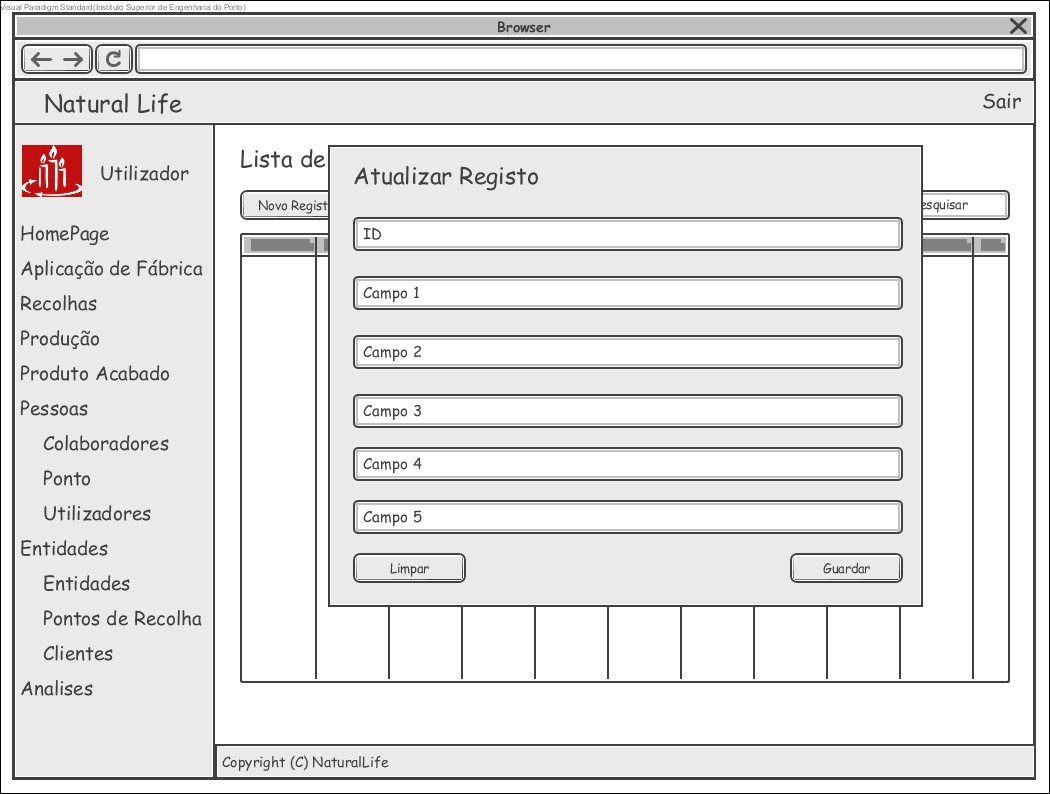
\includegraphics[width=0.60\textwidth,keepaspectratio]{figuras/Diagramas_vp/DI_Painel_3_Editar.jpg}
		\caption{Modelo da janela de edição na página de listagem}
		\label{fig:di_editar} 
	\end{center}
\end{figure}

\subsubsection*{Models compatíveis com o caso de uso}
Este caso de uso é compatível com os models Recolha, Produção, Produto Acabado, Colaboradores, Registo de Ponto, Entidades, Pontos de Recolha, Clientes e Analises.

\subsubsection*{Fluxo do caso de uso}
O caso de uso inicia-se quando o utilizador pressionar o botão editar da linha do registo que pretende atualizar. O sistema vai fazer um request em background para obter as informações da base de dados e apresenta uma janela flutuante com com os campos a serem pré-preenchidos com as informações recebidas. O utilizador faz as alterações que pretende e pressiona o botão guardar. Finalizado o registo a janela fecha-se e é apresentado uma mensagem ao utilizador.


\begin{figure}[H] 
	\begin{center}
		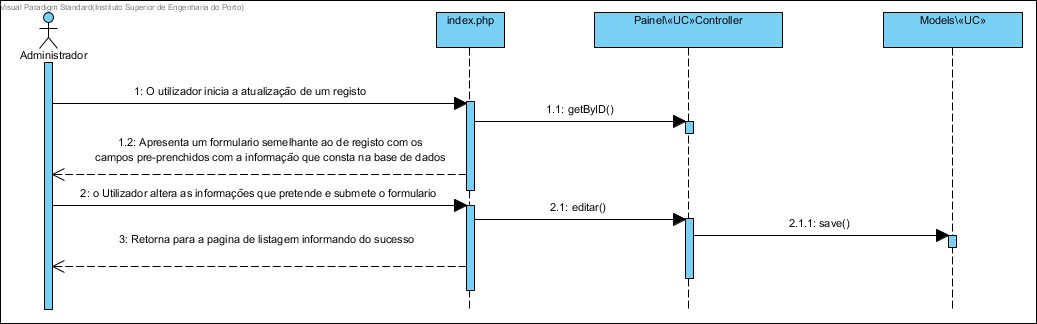
\includegraphics[width=\textwidth,keepaspectratio]{figuras/Diagramas_vp/SD_Painel_3_Editar.jpg}
		\caption{Diagrama de sequência de editar registo}
		\label{fig:sd_editar} 
	\end{center}
\end{figure}